% =============================================================================
% Appendix F: Wall-Clock Efficiency
% =============================================================================
\section{Wall-Clock Efficiency}\label{sec:wallclock}

\begin{table}[h]
\centering
\caption{Per-epoch wall-clock time (seconds) for 20-epoch training runs on a single RTX 5090 GPU.}
\label{tab:wallclock}
\small
\begin{tabular}{llcccc}
\toprule
Dataset & Architecture & Muon (s) & AdamW (s) & SGD (s) & Muon Overhead \\
\midrule
\multirow{3}{*}{CIFAR-100}
 & ResNet-50  & 58.8  & 53.4  & 53.2  & +10.1\% \\
 & DeiT-S     & 55.4  & 45.6  & 45.2  & +21.5\% \\
 & ConvNeXt-T & 116.8 & 106.9 & 107.1 & +9.3\%  \\
\midrule
\multirow{3}{*}{Tiny-ImageNet}
 & ResNet-50  & 118.2 & 99.5  & 96.5  & +18.8\% \\
 & DeiT-S     & 98.6  & 88.0  & 87.3  & +12.0\% \\
 & ConvNeXt-T & 219.2 & 208.2 & 205.6 & +5.3\%  \\
\midrule
\multirow{3}{*}{ImageNet-100}
 & ResNet-50  & 74.2  & 68.5  & 68.4  & +8.3\%  \\
 & DeiT-S     & 69.4  & 81.4$^\dagger$  & ---   & ---     \\
 & ConvNeXt-T & 134.4 & 122.5 & 123.6 & +9.7\%  \\
\bottomrule
\end{tabular}
\vspace{0.3em}
\par\noindent\footnotesize{Muon Overhead is computed relative to AdamW. $\dagger$\,DeiT-S AdamW on IN100 used a different batch configuration, making the timing comparison unreliable; IN100 DeiT-S SGD log was not found.}
\end{table}

\paragraph{Computational overhead of Newton-Schulz iteration.}
Muon's per-step cost exceeds AdamW by 5--22\% depending on architecture and dataset, attributable to the Newton-Schulz iteration used to approximate the matrix sign function for spectral-norm steepest descent. The overhead is largest on DeiT-S/CIFAR-100 (+21.5\%) where the parameter matrices are relatively small and the Newton-Schulz iterations dominate; it is smallest on ConvNeXt-T/Tiny-ImageNet (+5.3\%) where forward/backward pass computation amortizes the optimizer cost. SGD and AdamW have near-identical per-epoch times across all configurations, confirming that the overhead is specific to Muon's spectral decomposition.

% =============================================================================
% Appendix G: Alternative Spectral Optimizers
% =============================================================================
\section{Alternative Spectral Optimizers}\label{sec:alt_spectral}

\begin{table}[h]
\centering
\caption{Comparison of spectral optimizers on CIFAR-100 (20 epochs). Multi-seed means ($\pm$ std) reported where available; ConvNeXt-T SGD is single-seed (seed\,=\,42).}
\label{tab:spectral_comparison}
\small
\begin{tabular}{llcccc}
\toprule
 & & \multicolumn{4}{c}{Validation Accuracy (\%)} \\
\cmidrule(lr){3-6}
Architecture & & SOAP & Shampoo & Muon & AdamW \\
\midrule
ResNet-50  & & 77.28{\scriptsize$\pm$0.20} & 78.25{\scriptsize$\pm$0.18} & 76.88{\scriptsize$\pm$0.27} & 67.85{\scriptsize$\pm$0.17} \\
DeiT-S     & & 65.45{\scriptsize$\pm$0.18} & 63.53{\scriptsize$\pm$0.05} & 62.67{\scriptsize$\pm$0.41} & 52.33{\scriptsize$\pm$0.34} \\
ConvNeXt-T & & 74.40{\scriptsize$\pm$0.43} & 70.57{\scriptsize$\pm$0.29} & 74.62{\scriptsize$\pm$0.15} & 58.54{\scriptsize$\pm$2.17} \\
\bottomrule
\end{tabular}
\vspace{0.3em}
\par\noindent\footnotesize{Muon and AdamW values are multi-seed means ($\pm$ std), consistent with Table~\ref{tab:main_results}. SOAP is 3-seed; Shampoo is 3-seed on all architectures ($\text{lr}{=}7{\times}10^{-3}$ on ConvNeXt-T). All optimizers use per-architecture tuned learning rates from 5-epoch sweeps; Shampoo learning rates were refined via extended sweeps (Appendix~\ref{sec:hyperparams}).}
\end{table}

% =============================================================================
% Appendix I: Architecture Coverage Rationale
% =============================================================================
% =============================================================================
% Appendix: Layer-wise Spectral Analysis (Full)
% =============================================================================
\section{Layer-wise Spectral Analysis and Training Stability}\label{sec:spectral_analysis_full}

To localize where Muon's advantage arises within the network, we apply the weight swap protocol and spectral correlation analysis (Section~\ref{sec:method}) to CIFAR-100 models.

\paragraph{Weight Swap Results.}
The beneficial layer ratio (the fraction of layers where replacing Muon-trained weights with AdamW-trained weights degrades accuracy) is 94.3\% (50/53 layers) for ResNet-50 and 51.7\% (46/89 parameter groups) for DeiT-S.
Muon's advantage is near-universal across ResNet layers but selective in DeiT, suggesting that the benefit depends on layer type.

\paragraph{Spectral Divergence Correlations.}
Using checkpoints trained at independently selected optimal learning rates (Muon $\eta{=}0.02$, AdamW $\eta{=}10^{-3}$ for ResNet-50; Muon $\eta{=}0.003$, AdamW $\eta{=}10^{-4}$ for DeiT-S), we compute the Spearman rank correlation between per-layer stable rank divergence $\Delta \mathrm{sr}_l$ and per-layer Muon benefit $\Delta a_l$.
For ResNet-50, $\rho = +0.45$ ($p < 0.001$): layers where Muon and AdamW diverge most in stable rank tend to be the layers where Muon contributes the most.
For DeiT-S, the correlation reverses ($\rho = -0.40$, $p = 0.004$), confirming that the relationship between stable rank divergence and per-layer benefit is architecture-dependent: positive for CNNs, negative for transformers.

\paragraph{Training Stability Across Seeds.}

\begin{figure}[h]
\centering
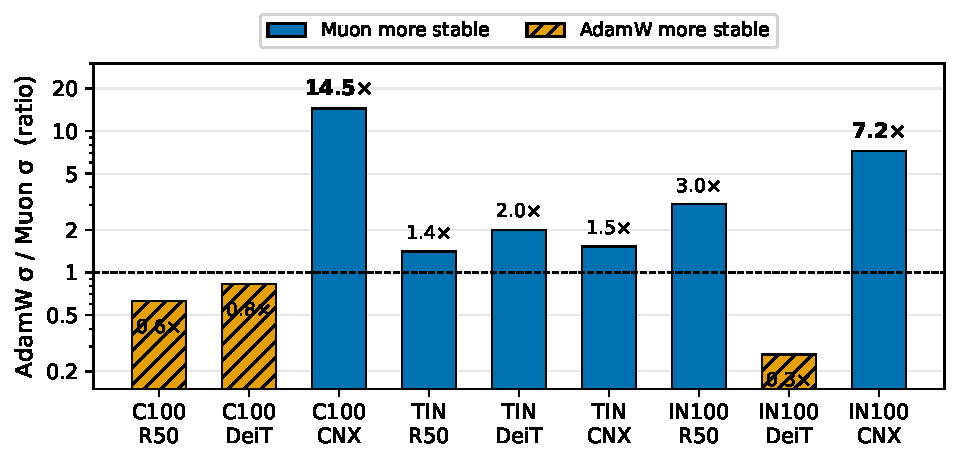
\includegraphics[width=\textwidth]{figures/fig3_stability.pdf}
\caption{Cross-seed standard deviation ($\sigma$) for Muon vs AdamW across all nine settings. Muon exhibits lower variance on 6/9 configurations; the stability advantage is architecture-dependent.}
\label{fig:stability}
\end{figure}

Cross-seed variance is architecture-dependent (Figure~\ref{fig:stability}): Muon shows substantially lower variance on convolutional architectures ($\sigma{=}0.15$ vs.\ $2.17$ on ConvNeXt-T/CIFAR-100), but AdamW is more stable on DeiT-S/ImageNet-100 ($\sigma{=}0.10$ vs.\ $0.38$).
Where Muon's variance reduction exceeds $7\times$ (ConvNeXt-T), fewer seeds suffice for reliable estimates.

% =============================================================================
% Appendix: Metric Robustness
% =============================================================================
\section{Metric Robustness}\label{sec:metric_robustness}

The sign reversal reported in Section~\ref{sec:spectral_analysis} is not an artifact of the chosen spectral metric. We verify this by computing the Spearman correlation between per-layer Muon benefit $\Delta a_l$ and three alternative divergence measures:

\begin{table}[h]
\centering
\caption{Spearman $\rho$ between per-layer divergence and Muon benefit under three spectral metrics. The sign reversal (positive on ResNet-50, negative on DeiT-S) is consistent across all metrics.}
\label{tab:metric_robustness}
\small
\begin{tabular}{@{}lcccc@{}}
\toprule
Metric & \multicolumn{2}{c}{ResNet-50} & \multicolumn{2}{c}{DeiT-S} \\
\cmidrule(lr){2-3} \cmidrule(lr){4-5}
 & $\rho$ & $p$ & $\rho$ & $p$ \\
\midrule
$\Delta\mathrm{sr}_l$ (stable rank) & $+0.45$ & ${<}0.001$ & $-0.40$ & $0.004$ \\
FCSB margin & $+0.40$ & ${<}0.01$ & $-0.51$ & ${<}0.001$ \\
$\Delta\mathrm{er}_l$ (effective rank) & $+0.43$ & ${<}0.01$ & $-0.33$ & $0.02$ \\
\bottomrule
\end{tabular}
\end{table}

All three metrics yield positive correlations on ResNet-50 and negative correlations on DeiT-S, confirming that the sign reversal is a robust structural phenomenon independent of the specific spectral measure.
We adopt stable rank as the primary metric because it is the most conservative (smallest $|\rho|$ on DeiT-S) and has favorable analytical properties: it is bounded, well-defined for rank-deficient matrices, and requires no architecture-specific normalization.

% =============================================================================
% Appendix: Normalization Swap Details
% =============================================================================
\section{Normalization Swap Implementation}\label{sec:normswap_details}

We replace all BatchNorm2d layers in ResNet-50 with GroupNorm(1, $C$), where $C$ is the number of channels.
GroupNorm with a single group computes statistics over all spatial and channel dimensions of each sample independently, making it equivalent to LayerNorm applied to convolutional feature maps~\cite{wu2018group}.
This substitution replaces 53 BatchNorm layers; all other architecture parameters, hyperparameters, and the training protocol remain identical to the standard ResNet-50 experiments (Section~\ref{sec:experimental_setup}).

% =============================================================================
% Appendix: Ablation Details
% =============================================================================
\section{Parameter Grouping Ablation Details}\label{sec:ablation_details}

The two-group AdamW ablation mirrors Muon's parameter routing exactly: 53 two-dimensional weight matrices ($23.45$M parameters, $\text{lr}{=}10^{-3}$) and 108 one-dimensional parameters ($0.26$M parameters, $\text{lr}{=}3{\times}10^{-4}$), with AdamW applied to both groups.
On ResNet-50 (CIFAR-100), two-group AdamW achieves $66.36 \pm 0.40\%$ ($n{=}3$, seeds 42/2/3), comparable to single-group AdamW ($67.85 \pm 0.17\%$) and far below Muon ($76.88 \pm 0.27\%$).
On ConvNeXt-T, two-group AdamW similarly matches standard AdamW ($59.44 \pm 0.28\%$ vs.\ $58.54 \pm 2.17\%$) while Muon maintains a $+15.2$\,pp advantage ($74.62 \pm 0.15\%$).
On DeiT-S, two-group AdamW degrades catastrophically to $30.08\%$ ($-22.3$\,pp vs.\ standard AdamW, single seed), as the reduced learning rate for 1D parameters (104/152 tensors in DeiT-S) severely undertrained LayerNorm parameters.

% =============================================================================
% Appendix I: Architecture Coverage Rationale
% =============================================================================
\section{Architecture Coverage in Supplementary Experiments}\label{sec:arch_coverage}

% =============================================================================
% Appendix: Additional Optimizer Comparisons
% =============================================================================
\section{Additional Optimizer Comparisons}\label{sec:additional_optimizers}

We evaluated Lion~\cite{chen2024lion} as a representative of sign-based optimizers to verify that the spectral family's advantage is not shared by all non-Adam methods.
On ResNet-50/CIFAR-100, Lion achieves $69.42\%$ (vs.\ AdamW $67.85\%$, $+1.57$\,pp), far below the spectral family ($+9$--$+10$\,pp over AdamW), confirming that the advantage is specific to spectral preconditioning rather than a general property of non-diagonal methods.
Other recent optimizers---Sophia~\cite{liu2024sophia} (diagonal Hessian clipping), Prodigy~\cite{mishchenko2024prodigy} (learning-rate-free estimation), GaLore~\cite{zhao2024galore} (low-rank gradient projection)---target computational cost or tuning difficulty rather than architecture robustness, making them complementary to rather than competitors of spectral methods.
A comprehensive comparison with these methods is left to future work.

% =============================================================================
% Appendix I: Architecture Coverage Rationale
% =============================================================================
\section{Architecture Coverage in Supplementary Experiments}\label{sec:arch_coverage}

The extended experiments in Appendix~\ref{sec:alt_spectral} focus on ResNet-50 and ConvNeXt-T rather than all three architectures from the main experiments. These two architectures represent the extremes of the normalization spectrum that drives Muon's variable effectiveness: ResNet-50 uses BatchNorm, where Muon's spectral updates interact with the implicit conditioning provided by BN; ConvNeXt-T uses LayerNorm, where the Muon--AdamW gap is largest (up to +24.30\,pp on IN100 at 20 epochs). DeiT-S, which also uses LayerNorm but in a pure self-attention architecture, exhibits intermediate gap magnitudes and is already thoroughly characterized across three datasets, three seed replicates, and two training horizons (20 and 50 epochs) in the main paper. Including DeiT-S in the supplementary experiments would add six additional training runs without meaningfully extending the analysis beyond the BN--LN axis already captured by the ResNet-50/ConvNeXt-T pair.

\section{Corruption Robustness}\label{sec:corruption_robustness}

We evaluate corruption robustness on CIFAR-100-C~\cite{hendrycks2019benchmarking}, which applies 19 corruption types at 5 severity levels to the CIFAR-100 test set. We report mean corruption error (mCE), normalized so that same-architecture, same-normalization AdamW = 100\%; lower is better.

\begin{table}[h]
\centering
\caption{Corruption robustness on CIFAR-100-C. mCE ($\downarrow$ is better) normalized so same-normalization AdamW = 100\%. Retention = corruption accuracy\,/\,clean accuracy, measuring inherent robustness independent of clean performance level.}
\label{tab:corruption_robustness}
\small
\begin{tabular}{llcccc}
\toprule
Architecture & Optimizer & Clean Acc (\%) & Corr Acc (\%) & mCE (\%) & Retention (\%) \\
\midrule
\multirow{4}{*}{ResNet-50 (BN)} & SOAP & 77.28 & 22.74 & \textbf{98.6} & 29.4 \\
 & Shampoo & 78.25 & 21.94 & 99.8 & 28.0 \\
 & AdamW & 67.85 & 22.40 & 100.0 & 33.0 \\
 & Muon & 76.88 & 21.59 & 100.5 & 28.1 \\
\midrule
\multirow{2}{*}{ResNet-50 (LN)} & Muon & 78.52 & 27.44 & \textbf{92.6} & 34.9 \\
 & AdamW & 50.51 & 22.93 & 100.0 & 45.4 \\
\midrule
\multirow{4}{*}{ConvNeXt-T} & Muon & 74.62 & 31.31 & \textbf{90.5} & 42.0 \\
 & SOAP & 74.40 & 26.23 & 99.1 & 35.3 \\
 & AdamW & 58.54 & 26.23 & 100.0 & 44.8 \\
 & Shampoo & 70.57 & 23.55 & 103.9 & 33.4 \\
\midrule
\multirow{4}{*}{DeiT-S} & Muon & 62.67 & 28.30 & \textbf{89.2} & 45.2 \\
 & SOAP & 65.45 & 21.47 & 98.3 & 32.8 \\
 & AdamW & 52.33 & 20.89 & 100.0 & 39.9 \\
 & Shampoo & 63.53 & 18.77 & 102.6 & 29.5 \\
\midrule
\multirow{5}{*}{ResNet-50 (GN32)} & Muon & 78.20 & 28.75 & \textbf{90.0} & 36.8 \\
 & SOAP & 75.52 & 27.88 & 91.3 & 36.9 \\
 & Shampoo & 74.79 & 26.96 & 92.6 & 36.0 \\
 & AdamW & 55.73 & 22.58 & 100.0 & 40.5 \\
 & SGD & 23.90 & 14.36 & 112.9 & 60.1 \\
\bottomrule
\end{tabular}
\end{table}

Muon achieves the lowest mCE on three of four architecture configurations (ConvNeXt-T: 90.5\%, DeiT-S: 89.2\%, ResNet-50-LN: 92.6\%), with the robustness advantage most pronounced on layer-normalized architectures. On ResNet-50 with BatchNorm, differences among optimizers are marginal (mCE 98.6--100.5\%), consistent with BatchNorm's known loss-landscape smoothing effect. Shampoo underperforms AdamW on ConvNeXt-T (mCE 103.9\%) and DeiT-S (102.6\%), while performing near-baseline on ResNet-50-BN (99.8\%), indicating that full-matrix Kronecker preconditioning does not translate to corruption robustness. Category-level analysis reveals that Muon's advantage concentrates in weather and digital corruptions (brightness, saturate, snow, frost, spatter), while noise corruptions (Gaussian, shot, impulse) show smaller inter-optimizer differences.

\paragraph{Dose-response pattern in corruption robustness.}
The GN(32) configuration extends the dose-response pattern observed in clean accuracy (Section~\ref{sec:norm_swap}) to corruption robustness. Under GN(32), all three spectral optimizers improve mean corruption accuracy by 5--7\,pp relative to their BN counterparts (Muon: $+7.2$\,pp, SOAP: $+5.1$\,pp, Shampoo: $+5.0$\,pp), while AdamW remains flat ($+0.2$\,pp). SGD under GN(32) degrades to 14.36\% mean corruption accuracy (mCE 112.9\%), an 8.2\,pp drop below GN(32) AdamW, mirroring the clean-accuracy collapse observed in the normalization-swap experiment. This three-way divergence---spectral methods improve, AdamW holds steady, SGD degrades---constitutes a dose-response pattern: as normalization smoothing is reduced from BN to GN(32), the optimizer's capacity for spectral preconditioning determines whether it can compensate for the lost implicit conditioning, in corruption robustness as in clean accuracy.
